\section{Coding}\label{code}
In this Appendix we reproduce all the quantities  that should be coded.

Eqs.~\eqref{calvimchiewn}, \eqref{calvimchie2wn}, \eqref{calvimchiwn}
 and \eqref{calvimchi2wn}
\begin{equation}\label{calvimchiewn}
\mathrm{Im}[\chi_{e,\rma\rmb\rmc,\go}^{s,\ell}] =
\frac{\pi |e|^3}{2\hbar^2}\sum_{vc\bfk}\sum_{l\neq(v,c)}\frac{1}{\omega^{S}_{cv}}
\left[
\frac{\mathrm{Im}[\mathcal{V}^{\gs,\text{a},\ell}_{lc}\{r^{\rmb}_{cv}r^{\rmc}_{vl}\}]}
{(2\go^\gs_{cv}-\go^\gs_{cl})} 
-\frac{\mathrm{Im}[\mathcal{V}^{\gs,\text{a},\ell}_{vl}\{r^{\rmc}_{lc}r^{\rmb}_{cv}\}]}
{(2\go^\gs_{cv}-\go^\gs_{lv})}
\right]\gd(\go^\gs_{cv}-\go),
\end{equation}  
\begin{equation}\label{calvimchiwn}
\mathrm{Im}[\chi_{i,\text{a}\text{b}\text{c},\omega}^{s,\ell}]
= \frac{\pi\vert e\vert^3}{2\hbar^2}\sum_{cv\mathbf{k}}\frac{1}{(\omega^{S}_{cv})^{2}}
\left[
\mathrm{Re}\left[\left\{r^{\text{b}}_{cv}\left(\mathcal{V}^{\gs,\text{a},\ell}_{vc}\right)_{;k^{\text{c}}}\right\}\right]
+\frac{\mathrm{Re}\left[\mathcal{V}^{\gs,\text{a},\ell}_{vc}\left\{r^{\text{b}}_{cv}
\Delta^{\text{c}}_{cv}\right\}\right]}{\omega^{S}_{cv}} 
\right]\delta(\omega^\gs_{cv}-\omega),
\end{equation}
\begin{equation}\label{calvimchie2wn}
\mathrm{Im}[\chi_{e,\rma\rmb\rmc,2\go}^{s,\ell}] =
-\frac{\pi |e|^3}{2\hbar^2}\sum_{vc\bfk}\frac{4}{\omega^{S}_{cv}}
\left[
\sum_{v'\ne
  v}\frac{\mathrm{Im}[\mathcal{V}^{\gs,\text{a},\ell}_{vc}\{r^{\rmb}_{cv'}r^{\rmc}_{v'v}\}]}
{2\go^\gs_{cv'}-\go^\gs_{cv}}
- \sum_{c'\ne
  c}\frac{\mathrm{Im}[\mathcal{V}^{\gs,\text{a},\ell}_{vc}\{r^{\rmc}_{cc'}r^{\rmb}_{c'v}\}]}
{2\go^\gs_{c'v}-\go^\gs_{cv}}
\right]\gd(\go^\gs_{cv}-2\go),
\end{equation}
and
\begin{equation}\label{calvimchi2wn}
\mathrm{Im}[\chi_{i,\text{a}\text{b}\text{c},2\omega}^{s,\ell}] 
=
 \frac{\pi \vert
   e\vert^{3}}{2\hbar^2}\sum_{vc\mathbf{k}}\frac{4}{(\omega^{S}_{cv})^{2}}
\left[\mathrm{Re}\left[\mathcal{V}^{\gs,\text{a},\ell}_{vc}\left\{\left(r^{\text{b}}_{cv}\right)_{;k^{\text{c}}}
\right\}\right] -
\frac{2\mathrm{Re}\left[\mathcal{V}^{\gs,\text{a},\ell}_{vc}\left\{r^{\text{b}}_{cv}
\Delta^{\text{c}}_{cv}\right\}\right]}{\omega^{S}_{cv}}\right]\delta(\omega^\gs_{cv}-2\omega)
,
\end{equation}


\noindent$\bullet$ Coding:
$\calv^{\gs,\rma,\ell}_{nm}\to$ \verb=calVsig=,
$r^\rma_{nm}\to$ \verb=posMatElem=,
$\left(\calv^{\gs,\rma,\ell}_{nm}\right)_{;k^\rmb}\to$ \verb=gdcalVsig=,
and\\ $(r^\rma_{nm})_{;k^\rmb}\to$ \verb=derMatElem=

$\bullet$ proof:\\
To evaluate above expressions we need the following ($m_e=1$):
\begin{align}\label{}
\bfv^\lda_{nm}(\bfk) 
=(1/m_e)\bfp_{nm}(\bfk)+\bfv^\nl_{nm}(\bfk)
=\bfp_{nm}(\bfk)+\bfv^\nl_{nm}(\bfk)
,
\end{align}
that
 includes the local and nonlocal parts of the pseudopotential. They
 correspond to the following files:\\
$\bullet$ $\bfp_{nm}(\bfk)\to$ \verb=me_pmn_*=\\
$\bullet$ $\bfv^\nl_{nm}(\bfk)\to$ \verb=me_vnlnm_*=\\
where the \verb=nm= or \verb=mn= order in the files is irrelevant, and
ought to be fixed just for the {\it biuty} of it.
Option \verb=-n= in \verb=all_responses.sh= does
\begin{enumerate}
\item 
 \verb=> cp me_pmn_* me_pmn_*.o= 
\item adds \verb=me_pmn_*= and \verb=me_vnlnm_*= into
  \verb=me_pmn_*= 
\item calculates the response
\item \verb=> mv me_pmn_*.o me_pmn_*=
\end{enumerate}
so   
$\bfv^\lda_{nm}(\bfk)$, stored in \verb=vldaMatElem=
is available for the calculation of the response, and with it we calculate
(Eqs.~\eqref{chon.9} and \eqref{chon.10}),
\begin{align}\label{c-chon.98}
\bfv^\gs_{nm}(\bfk)
&=
\left(1+\frac{\gS}{\go_c(\bfk)-\go_v(\bfk)}\right)\bfv^\lda_{nm}(\bfk)
\quad\quad n\notin D_m
\nonumber\\
\bfv^\gs_{nn}(\bfk)
&=
\bfv^\lda_{nn}(\bfk)
\nonumber\\
\bfr_{nm}(\bfk)&=\frac{\bfv^\gs_{nm}(\bfk)}{i\go^\gs_{nm}(\bfk)}
=\frac{\bfv^\lda_{nm}(\bfk)}{i\go^\lda_{nm}(\bfk)}
\quad\quad n\notin D_m
.
\end{align}   
If option \verb=-n= is not chosen, then the contribution of $\bfv^\nl_{nm}(\bfk)$
is neglected in the calculation of any response. Obviously, in this
case the code only uses \verb=me_pmn_*= without adding \verb=me_vnlnm_*= 

We need Eq.~\eqref{a.1} and \eqref{a.2}
\begin{align}\label{c-a.1}
\calv^{\gs,\rma,\ell}_{nm}
&=
\calv^{\lda,\rma,\ell}_{nm}
+
\calv^{\cals,\rma,\ell}_{nm}
\nonumber\\
\left(
\calv^{\gs,\rma,\ell}_{nm}
\right)_{;k^\rmb}
&=
\left(
\calv^{\lda,\rma,\ell}_{nm}
\right)_{;k^\rmb}
+
\left(
\calv^{\cals,\rma,\ell}_{nm}
\right)_{;k^\rmb}
.
\end{align}
 The first LDA term is
\begin{align}\label{c-a.2}
\calv^{\lda,\rma,\ell}_{nm}
&=
\frac{1}{2}\sum_q\left(
v^{\lda,\rma}_{nq}\calc^\ell_{qm}+\calc^\ell_{nq} v^{\lda,\rma}_{qm}
\right)
.
\end{align} 
If option \verb=-n= is not chosen in \verb=all_responses.sh=
Eq.~\eqref{c-a.2}
 is
not calculated and\\
$\bullet$ $\calv^{\lda,\rma,\ell}_{nm}\to$ \verb=me_cpmn_*=\\  
If option \verb=-n= is chosen Eq.~\eqref{c-a.2}
 must be calculated as given in
\verb=set_input_ascii.f90=. We mention that
$\calv^{\lda,\rma,\ell}_{nm}$ can be computed directly,\cite{nicolaspc}
avoiding the sum over the full set of bands $q$, however we chose to
compute Eq.~\eqref{c-a.2}, which is done in
\verb=functions.f90=.
Then, we need 
Eq.~\eqref{eni.4}
\begin{align}\label{c-eni.4}
\calc^\ell_{nm}(\bfk)&=
\sum_{\bfG,\bfG'} A^*_{n\bfk}(\bfG')  A_{m\bfk}(\bfG)
\gd_{\bfG_\parallel \bfG'_\parallel}
f_\ell(G_\perp-G'_\perp)
\nonumber\\
\calc^\ell_{mn}(\bfk)&=
\big(\calc^\ell_{nm}(\bfk)\big)^*
,
\end{align} 
which is coded in \verb=sub_pmn_ascii.f90= within the same subroutine of $\calbv^\ell_{nm}$
calculated with Eq.~\eqref{eni.2}. However, Sean out of the blue, call
it \verb=me_cfmn_*= in \verb=run_tiniba.sh=,
 and Darwin won (what else? ID??), 
thus I call it \verb=cfMatElem= in \verb=SRC_1setinput=. ID would call
it  \verb=ccMatElem=
but long live CD!

 The second LDA term is
\begin{align}\label{c-a.2n}
\left(\calv^{\lda,\rma,\ell}_{nm}\right)_{;k^\rmb}
&=
\frac{1}{2}\sum_q\left(
(v^{\lda,\rma}_{nq})_{;k^\rmb}\calc^\ell_{qm}
+  
v^{\lda,\rma}_{nq}(\calc^\ell_{qm})_{;k^\rmb}
+
(\calc^\ell_{nq})_{;k^\rmb} v^{\lda,\rma}_{qm}
+
\calc^\ell_{nq} (v^{\lda,\rma}_{qm})_{;k^\rmb}
\right)
,
\end{align}  
where\\
$\bullet$ for $n\ne m$\\
Eq.~\eqref{a.3}
\begin{align}\label{c-a.3}
(v^{\lda,\rma}_{nm})_{;k^\rmb}
&=  
im_e\left(\gD^b_{nm}r^\rma_{nm}
+ 
\go^\lda_{nm}(r^\rma_{nm})_{;k^\rmb}
\right)
\nonumber\\
(v^{\lda,\rma}_{mn})_{;k^\rmb}
&=
\left((v^{\lda,\rma}_{nm})_{;k^\rmb}\right)^*
\quad\mathrm{for}\quad n\ne m
,
\end{align} 
with
Eq.~\eqref{eli.13}
\begin{align}\label{c-eli.13}
\gD_{nm}^{\rma}
=
v_{nn}^{\lda,\rma}-v_{mm}^{\lda,\rma}
,
\end{align}
and \eqref{na_rgendevn}
\begin{align}\label{c-na_rgendevn}
(r^{\rmb}_{nm})_{;k^{\rma}}
&=
-i\calt^{\rma\rmb}_{nm}
+
\frac{
r^{\rma}_{nm}
\Delta^{\rmb}_{mn}
+r^{\rmb}_{nm}
\Delta^{\rma}_{mn}
}
{\go^\lda_{nm}}
+
\frac{i}{\go^\lda_{nm}}
\sum_{\ell}
\bigg(
\go^\lda_{\ell m}
r^{\rma}_{n\ell}
r^{\rmb}_{\ell m}
-
\go^\lda_{n\ell}
r^{\rmb}_{n\ell}
r^{\rma}_{\ell m}
\bigg)
\nonumber\\
&\approx
\frac{
r^{\rma}_{nm}
\Delta^{\rmb}_{mn}
+r^{\rmb}_{nm}
\Delta^{\rma}_{mn}
}
{\go^\lda_{nm}}
+
\frac{i}{\go^\lda_{nm}}
\sum_{\ell}
\bigg(
\go^\lda_{\ell m}
r^{\rma}_{n\ell}
r^{\rmb}_{\ell m}
-
\go^\lda_{n\ell}
r^{\rmb}_{n\ell}
r^{\rma}_{\ell m}
\bigg)
\nonumber\\
(r^{\rmb}_{mn})_{;k^{\rma}}
&=
\left((r^{\rmb}_{nm})_{;k^{\rma}}\right)^*
,
\end{align}
where $\calt^{\rma\rmb}_{nm}\approx 0$.\\
$\bullet$ for $n=m$\\
Since 
$\calt^{\rma\rmb}_{nn}\approx (\hbar/m_e)\gd_{\rma\rmb}$,
Eq.~\eqref{a.3c} gives
\begin{align}\label{c-a.3c}
(v^{\lda,\rma}_{nn})_{;k^\rmb}
&=
-i\calt^{\rma\rmb}_{nn}
-
\sum_{\ell\ne n}
\go^\lda_{\ell n}
\bigg( 
r^{\rma}_{n\ell} 
r^\rmb_{\ell n}
+ 
r^\rmb_{n\ell} 
r^{\rma}_{\ell n}
\bigg)
\nonumber\\
&\approx
\frac{\hbar}{m_e}\gd_{\rma\rmb}
-
\sum_{\ell\ne n}
\go^\lda_{\ell n}
\bigg( 
r^{\rma}_{n\ell} 
r^\rmb_{\ell n}
+ 
r^\rmb_{n\ell} 
r^{\rma}_{\ell n}
\bigg)
.
\end{align} 
For Eq.~\eqref{c-a.2n} we need
\eqref{a.7}
\begin{align}\label{c-a.7}
 (\calc^\ell_{nm})_{;k^\rma}
&= 
i\sum_{q\ne nm}
\left(
r_{nq}^\rma
\calc^\ell_{qm}
-
\calc^\ell_{nq}
r_{qm}^\rma
\right)
+ir_{nm}^\rma(\calc^\ell_{mm}-\calc^\ell_{nn})
\nonumber\\
 (\calc^\ell_{mn})_{;\bfk}
&=
\big( (\calc^\ell_{nm})_{;\bfk}\big)^*
.
\end{align} 

For the scissor related term we have:
Eq.~\eqref{a.3b} , \eqref{choni.1} and \eqref{chon.2}
\begin{align}\label{c-a.3b}
\calv^{\cals,\rma,\ell}_{nm}
&=
\frac{1}{2}\sum_q\left(  
v^{\cals,\rma}_{nq}\calc^\ell_{qm}+\calc^\ell_{nq} v^{\cals,\rma}_{qm}
\right)
\nonumber\\
\left(\calv^{\cals,\rma,\ell}_{nm}\right)_{;k^\rmb}
&=
\frac{1}{2}\sum_q\left(
(v^{\cals,\rma}_{nq})_{;k^\rmb}\calc^\ell_{qm}
+   
v^{\cals,\rma}_{nq}(\calc^\ell_{qm})_{;k^\rmb}
+
(\calc^\ell_{nq})_{;k^\rmb} v^{\cals,\rma}_{qm}
+
\calc^\ell_{nq} (v^{\cals,\rma}_{qm})_{;k^\rmb}
\right)
,
\end{align}   
with Eqs.~\eqref{chon.2} and \eqref{choni.1}
\begin{align}\label{c-chon.2} 
v^{\cals,\rma}_{nm}=i\gS f_{mn}r^\rma_{nm}
,
\end{align}
\begin{align}\label{c-choni.1}
(v^{\cals,\rma}_{nm})_{;k^\rmb}=
i\gS f_{mn}(r^\rma_{nm})_{;k^\rmb}
,
\end{align}
where $\hbar\gS$ is the scissors correction.
Notice that
$v^{\cals,\rma}_{nn}=0$ and 
$(v^{\cals,\rma}_{nn})_{;k^\rmb}=0$.
Substuiting Eq.~\eqref{c-chon.2} into \eqref{c-a.3b}, we obtain
  \begin{align}\label{vs.vc}
      \mathcal{V}^{S,a,\ell}_{vc}
&= 
      -\frac{i\Sigma}{2}
      \left[\sum_{v^{\prime}}r^{a}_{vv^{\prime}}C^{\ell}_{v^{\prime}c} 
          +
          \sum_{c^{\prime}}C^{\ell}_{vc^{\prime}}r^{a}_{c^{\prime}c}\right],
\quad\quad\mathrm{Coded}
\nonumber\\
      \mathcal{V}^{S,a,\ell}_{cv}
&= 
      \frac{i\Sigma}{2}
      \left[\sum_{v^{\prime}}r^{a}_{cv^{\prime}}C^{\ell}_{v^{\prime}v} 
          + \sum_{c^{\prime}}C^{\ell}_{cc^{\prime}}r^{a}_{c^{\prime}v}\right],
\nonumber\\
      \mathcal{V}^{S,a,\ell}_{cv}
&= 
      (\mathcal{V}^{S,a,\ell}_{vc})^*
    \end{align}
and    
  \begin{align}\label{vs.cc}
    \mathcal{V}^{S,a,\ell}_{cc} 
    &= -\Sigma\sum_{v}
    \text{Im}\left[r^{a}_{cv}C^{\ell}_{vc}\right],
  \end{align}
 \begin{align}\label{vs.vv}
    \mathcal{V}^{S,a,\ell}_{vv} 
    &= \Sigma\sum_{c}
    \text{Im}\left[r^{a}_{vc}C^{\ell}_{cv}\right],
  \end{align}
where the last two are real functions as they must, since they are
velocities, and are coded in:\\
$\bullet$ Coding: \verb=functions.f90= array \verb=calVscissors=

Substuiting Eqs.~\eqref{c-chon.2} and \eqref{c-choni.1} into \eqref{c-a.3b}, we obtain
\begin{align}\label{dgvs.cv}
\left(\calv^{\cals,\rma\,\ell}_{cv}\right)_{;k^\rmb}
&=
\frac{i\gS}{2}
\left(
\sum_{v'}\left(
 (r^\rma_{cv'})_{;k^\rmb}\calc^\ell_{v'v}
+  
r^\rma_{cv'}(\calc^\ell_{v'v})_{;k^\rmb}
\right)
+
\sum_{c'}\left(
(\calc^\ell_{cc'})_{;k^\rmb} r^\rma_{c'v}
+
\calc^\ell_{cc'} (r^\rma_{c'v})_{;k^\rmb}
\right)
\right)
\nonumber\\
\left(\calv^{\cals,\rma,\ell}_{vc}\right)_{;k^\rmb}
&=
\left(\left(\calv^{\cals,\rma,\ell}_{cv}\right)_{;k^\rmb}\right)^*
,
\end{align}  
\begin{align}\label{dgvs.cc}
\left(\calv^{\cals,\rma,\ell}_{cc}\right)_{;k^\rmb}
&=
-\gS
\sum_{v}
 \mathrm{Im}\left[(r^\rma_{cv})_{;k^\rmb}\calc^\ell_{vc}
+
r^\rma_{cv}
(\calc^\ell_{vc}) _{;k^\rmb}\right]
,
\end{align}  
and
\begin{align}\label{dgvs.vv}
\left(\calv^{\cals,\rma,\ell}_{vv}\right)_{;k^\rmb}
&=
\gS
\sum_{c}
 \mathrm{Im}\left[(r^\rma_{vc})_{;k^\rmb}\calc^\ell_{cv}
+
r^\rma_{vc}(\calc^\ell_{cv}) _{;k^\rmb}\right]
.
\end{align}  
$\bullet$ Coding:\\
$(r^\rma_{nm})_{;k^\rmb}\to$ \verb=derMatElem=
$\calc^\ell_{nm}\to$ \verb=cfMatElem=
$r^\rma_{nm}\to$ \verb=posMatElem=
$(\calc^\ell_{nm})_{;k^\rmb}\to$ \verb=gdf=, and\\
$\left(\calv^{\cals,\rma,\ell}_{nm}\right)_{;k^\rmb}\to$ 
\verb=gdcalVS=

\subsection{Coding for $\calv^{\gs,\rma,\ell}_{nm}(\bfk)$} 
Recall that 
$\calv^{\lda,\rma,\ell}_{mn}=(\calv^{\lda,\rma,\ell}_{nm})^*$
and 
$\calv^{\cals,\rma,\ell}_{mn}=(\calv^{\cals,\rma,\ell}_{nm})^*$ 
\begin{itemize}
%%%
\item If \verb=-n= option is chosen in \verb=all_responses.sh=
\begin{itemize}
\item $\calv^{\lda,\rma,\ell}_{nm}$, comes from
  Eq.~\eqref{c-a.2}, coded in \verb=functions.f90=
\end{itemize}
%%%
\item If \verb=-n= option is NOT chosen in \verb=all_responses.sh=
\begin{itemize}
\item $\calv^{\lda,\rma,\ell}_{nm}$ 
is used from \verb=me_cpmn_*=
  which is Eq.~\eqref{eni.2} and is coded in \verb=sub_pmn_ascii.f90=
\end{itemize}
%%%
\end{itemize}
For either case
\begin{itemize}
\item $\calv^{\cals,\rma,\ell}_{nm}$ 
is obtained from
  Eqs.~\eqref{vs.vc}, \eqref{vs.cc} or \eqref{vs.vv}, depending on
  $nm$. This is coded in \verb=functions.f90= and used in 
\verb=set_input_ascii.f90=  
\end{itemize}
Thus,\\
$\bullet$ 
$\calv^{\gs,\rma,\ell}_{nm}(\bfk)=\calv^{\lda,\rma,\ell}_{nm}(\bfk)+\calv^{\cals,\rma,\ell}_{nm}(\bfk)$\\ 
is stored in \verb=calMomMatElem=  
array, constructed in 
\verb=set_input_ascii.f90=, and used in \verb=SRC_2latm= for
integrating the response function. A brave young soul, should change   
\verb=calMomMatElem= to \verb=calVelMatElem= in order to have a more
appropriate name. But as good old DNA, we construct upon available
ATGC; using the old structure, adding functionality and  keeping all
the usles non-codifying crap, thus making Darwin
 proud of us! 

\subsection{Coding for $(\calv^{\gs,\rma,\ell}_{nm}(\bfk))_{;k^\rmb}$}
\begin{itemize}
\item $\gD^\rma_{nm}$ available in array \verb=Delta=, 
calculated in \verb=set_input_ascii.f90=,
 and contains the
  contribution from $\bfv^\nl_{nm}(\bfk)$ if the \verb=-n= option is
  chosen in \verb=all_responses.sh= 
\item $(r^\rma_{nm}(\bfk))_{;k^\rmb}$
 available in array
  \verb=derMatElem=,
calculated in \verb=set_input_ascii.f90= and \verb=functions.f90=,
 and contains the
  contribution from $\bfv^\nl_{nm}(\bfk)$ if the \verb=-n= option is
  chosen in \verb=all_responses.sh= 
\item With above two we compute $(v^{\lda,\rma}_{nm}(\bfk))_{;k^\rmb}$ 
in \verb=set_input_ascii.f90=  and store it in \verb=gdVlda= for
diagonal and off diagonal terms.
\item $\big(\calc^\ell_{nm}(\bfk)\big)_{;k^\rma}$ is coded in 
in \verb=set_input_ascii.f90=  and store it in \verb=gdf= for
diagonal and off diagonal terms. Darwin at work!
\item $(v^{\lda,\rma}_{nq})_{;k^\rmb}\to$ \verb=gdVlda=,
  $\calc^\ell_{qm}\to$ \verb=cfMatElem=,
$v^{\lda,\rma}_{nq}\to$ \verb=vldaMatElem=, 
$(\calc^\ell_{qm})_{;k^\rmb}\to$
\verb=gdf=

 \begin{align}\label{c-a.2nn}
\left(\calv^{\lda,\rma,\ell}_{nm}\right)_{;k^\rmb}
&=
\frac{1}{2}\sum_q\left(
(v^{\lda,\rma}_{nq})_{;k^\rmb}\calc^\ell_{qm}
+ 
v^{\lda,\rma}_{nq}(\calc^\ell_{qm})_{;k^\rmb}
+
(\calc^\ell_{nq})_{;k^\rmb} v^{\lda,\rma}_{qm}
+
\calc^\ell_{nq} (v^{\lda,\rma}_{qm})_{;k^\rmb}
\right)
\nonumber\\
\left(\calv^{\lda,\rma,\ell}_{mn}\right)_{;k^\rmb}&=\left(\left(\calv^{\lda,\rma,\ell}_{nm}\right)_{;k^\rmb}\right)^*
,
\end{align} 
$\left(\calv^{\lda,\rma,\ell}_{nm}\right)_{;k^\rmb}\to$
\verb=gdcalVlda= and coded in \verb=set_input_ascii.f90=
\end{itemize}

\subsection{Summary}
\begin{itemize}
\item
$\calv^{\gs,\rma,\ell}_{nm}(\bfk)=\calv^{\lda,\rma,\ell}_{nm}(\bfk)+\calv^{\cals,\rma,\ell}_{nm}(\bfk)\to$
\verb=calMomMatElem= 

\item $\left(\calv^{\lda,\rma,\ell}_{nm}\right)_{;k^\rmb}\to$
\verb=gdcalVlda= 

\item $\left(\calv^{\cals,\rma,\ell}_{nm}\right)_{;k^\rmb}\to$ 
\verb=gdcalVS=

\item $\left(\calv^{\gs,\rma,\ell}_{nm}\right)_{;k^\rmb}=
\left(\calv^{\lda,\rma,\ell}_{nm}\right)_{;k^\rmb}+\left(\calv^{\cals,\rma,\ell}_{nm}\right)_{;k^\rmb}\to$ 
\verb=gdcalVsig=
\end{itemize}

\subsection{Bulk expressions}

For a bulk $\calc^\ell_{nm}(\bfk)=\gd_{nm}$, then
$(\calc^\ell_{nm}(\bfk))_{;\bfk}=0$, and Eq.~\eqref{c-a.1} reduces to
\begin{align}\label{choni.9}
v^{\gs,\rma}_{nm}
&=
v^{\lda,\rma}_{nm}
+
v^{\cals,\rma}_{nm}
\nonumber\\
\bfv^\gs_{nm}(\bfk)
&=
\left(1+\frac{\gS}{\go_c(\bfk)-\go_v(\bfk)}\right)\bfv^\lda_{nm}(\bfk)
\quad\quad n\notin D_m
\nonumber\\
\bfv^\gs_{nn}(\bfk)
&=
\bfv^\lda_{nn}(\bfk)
,
\end{align}
where in \verb=$TINIBA/latm= the values are coded in the array
called
\verb=momMatElem=.  
If option \verb=-n= is given while running
\verb=all_resposnses.sh=, then $\bfv^\nl_{nm}(\bfk)$ are included in 
\verb=momMatElem=. 
Also,
\begin{align}\label{c-a.1nn}
\left(v^{\gs,\rma}_{nm}\right)_{;k^\rmb}
&=
\left(
v^{\lda,\rma}_{nm}
\right)_{;k^\rmb}
+
\left(
v^{\cals,\rma}_{nm}
\right)_{;k^\rmb}
\nonumber\\
&=
\left(
v^{\lda,\rma}_{nm}
\right)_{;k^\rmb}
+
i\gS f_{mn}(r^\rma_{nm})_{;k^\rmb}
\nonumber\\
\left(v^{\gs,\rma}_{mn}\right)_{;k^\rmb}
&=
\left(\left(v^{\gs,\rma}_{nm}\right)_{;k^\rmb}\right)^*
,
\end{align}
where with the r.h.s. expressions are given above. 

$\bullet$ Coding:
$\bfv^\gs_{nm}(\bfk)\to$ \verb=momMatElem=,
$\left(v^{\lda,\rma}_{nm}\right)_{;k^\rmb}\to$ \verb=gdVlda=,
$\left(r^{\lda,\rma}_{nm}\right)_{;k^\rmb}\to$ \verb=derMatElem=, and
$\left(v^{\gs,\rma}_{nm}\right)_{;k^\rmb}\to$ \verb=gdVsig=

\subsection{Layer or Bulk calculation}
\begin{itemize}
\item Layer: The layer calculation is done by using
Eqs.~\eqref{c-calvimchiewn}, \eqref{c-calvimchie2wn}, \eqref{c-calvimchiwn}
 and \eqref{c-calvimchi2wn}. 
\item Bulk:
A bulk calculation can be performed by using the same
Eqs.~\eqref{c-calvimchiewn}, \eqref{c-calvimchie2wn}, \eqref{c-calvimchiwn}
 and \eqref{c-calvimchi2wn}, and by simply replacing
\begin{enumerate}
\item $\calbv^\gs_{nm}$ (\verb=calMomMatElem=) $\to \bfv^\gs_{nm}$ (\verb=momMatElem=) 
\item $(\calbv^\gs_{nm})_{;\bfk}$ (\verb=gdcalVsig=) $\to
  (\bfv^\gs_{nm})_{;\bfk}$ (\verb=gdVsig=) 
\end{enumerate}
\item Therefore: For the code to run either possibility we use the
  same arrays as for the layered response, where, if bulk is chosen, it
  simply copies the bulk matrix elements into the layer arrays, i.e.
\begin{itemize}
\item Layer: 
$\calbv^\gs_{nm}$ (\verb=calMomMatElem=) and
$(\calbv^\gs_{nm})_{;\bfk}$ (\verb=gdcalVsig=) 
\item Bulk:
$\bfv^\gs_{nm}$ (\verb=momMatElem=$\to$\verb=calVsig=) and
$(\bfv^\gs_{nm})_{;\bfk}$ (\verb=gdVsig=$\to$\verb=gdcalVsig=) \\
This change is done in \verb=set_input_ascii.f90= (look for
\verb=layer-to-bulk= tag)
\item ID: Notice that we have assigned\\
  \verb=calMomMatElem=$\to$ \verb=calVsig= (keeping
  \verb=calMomMatElem=), so it is easier to  code the responses.
Therefore, we have\\
$\calbv^\gs_{nm}\to$ \verb=calVsig= and
$(\calbv^\gs_{nm})_{;\bfk}\to$ \verb=gdcalVsig=\\
either for bulk or layered response. \\
If \verb=calMomMatElem= is not used, we should get rid of it (ID at work).
\end{itemize}
\end{itemize}

\subsection{$\calv$ vs ${\cal R}$}

Using 
$\mathrm{Re}[iz]=-\mathrm{Im}[z]$,
$\mathrm{Im}[iz]=\mathrm{Re}[z]$,
and
\begin{equation}\label{rnmenm91}
{\cal R}^\rma_{nm}=\frac{{\cal P}^\rma_{nm}}{im_e\go_{nm}}
\quad\quad n\ne m
,
\end{equation}
we can show the equivalence between the two formulations, i.e.
\begin{align}\label{imchiew}
\mathrm{Im}[\chi_{e,\rma\rmb\rmc,\go}^{s,\ell}]
&=
\frac{\pi |e|^3}{2\hbar^2} 
\sum_{vc\bfk}
\sum_{l\neq(v,c)}
\left[
\frac{\go^S_{lc}\mathrm{Re}[{\cal R}^{\rma,\ell}_{lc}\{r^{\rmb}_{cv}r^{\rmc}_{vl}\}]}
{\go^S_{cv}(2\go^S_{cv}-\go^S_{cl})}
-
\frac{\go^S_{vl}\mathrm{Re}[{\cal R}^{\rma,\ell}_{vl}\{r^{\rmc}_{lc}r^{\rmb}_{cv}\}]}
{\go^S_{cv}(2\go^S_{cv}-\go^S_{lv})}
\right]
\gd(\go^S_{cv}-\go)
,
\end{align}  
\begin{equation}\label{c-calvimchiewn}
\mathrm{Im}[\chi_{e,\rma\rmb\rmc,\go}^{s,\ell}] =
\frac{\pi |e|^3}{2\hbar^2}\sum_{vc\bfk}\sum_{l\neq(v,c)}\frac{1}{\omega^{S}_{cv}}
\left[
\frac{\mathrm{Im}[\mathcal{V}^{\gs,\text{a},\ell}_{lc}\{r^{\rmb}_{cv}r^{\rmc}_{vl}\}]}
{(2\go^\gs_{cv}-\go^\gs_{cl})} 
-\frac{\mathrm{Im}[\mathcal{V}^{\gs,\text{a},\ell}_{vl}\{r^{\rmc}_{lc}r^{\rmb}_{cv}\}]}
{(2\go^\gs_{cv}-\go^\gs_{lv})}
\right]\gd(\go^\gs_{cv}-\go),
\end{equation}  
\begin{align}\label{imchiwf}
\mathrm{Im}[\chi_{i,\rma\rmb\rmc,\go}^{s,\ell}]
&=
\frac{\pi|e|^3}{2\hbar^2}
\sum_{cv\bfk}
\frac{1}{\go^S_{cv}}
\left[
\mathrm{Im}[\{r^{\rmb}_{cv}\left({\cal R}^{\rma,\ell}_{vc}\right)_{;k^{\rmc}}\}]
+
\frac{2\mathrm{Im}[{\cal R}^{\rma,\ell}_{vc}\{r^{\rmb}_{cv}\gD^{\rmc}_{cv}\}]}{\go^S_{cv}}
\right]
\gd(\go^S_{cv}-\go)
,
\end{align}
\begin{equation}\label{c-calvimchiwn}
\mathrm{Im}[\chi_{i,\text{a}\text{b}\text{c},\omega}^{s,\ell}]
= \frac{\pi\vert e\vert^3}{2\hbar^2}\sum_{cv\mathbf{k}}\frac{1}{(\omega^{S}_{cv})^{2}}
\left[
\mathrm{Re}\left[\left\{r^{\text{b}}_{cv}\left(\mathcal{V}^{\gs,\text{a},\ell}_{vc}\right)_{;k^{\text{c}}}\right\}\right]
+\frac{\mathrm{Re}\left[\mathcal{V}^{\gs,\text{a},\ell}_{vc}\left\{r^{\text{b}}_{cv}
\Delta^{\text{c}}_{cv}\right\}\right]}{\omega^{S}_{cv}} 
\right]\delta(\omega^\gs_{cv}-\omega),
\end{equation}
\begin{align}\label{imchie2w}
\mathrm{Im}[\chi_{e,\rma\rmb\rmc,2\go}^{s,\ell}]
&=
\frac{\pi |e|^3}{2\hbar^2} 
\sum_{vc\bfk} 
4
\left[
\sum_{v'\ne v}
\frac{\mathrm{Re}[{\cal
    R}^{\rma,\ell}_{vc}\{r^{\rmb}_{cv'}r^{\rmc}_{v'v}\}]}{2\go^S_{cv'}-\go^S_{cv}}
-
\sum_{c'\ne c}
\frac{\mathrm{Re}[{\cal R}^{\rma,\ell}_{vc}\{r^{\rmc}_{cc'}r^{\rmb}_{c'v}\}]}
{2\go^S_{c'v}-\go^S_{cv}}
\right]
\gd(\go^S_{cv}-2\go)
,
\end{align}  
\begin{equation}\label{c-calvimchie2wn}
\mathrm{Im}[\chi_{e,\rma\rmb\rmc,2\go}^{s,\ell}] =
-\frac{\pi |e|^3}{2\hbar^2}\sum_{vc\bfk}\frac{4}{\omega^{S}_{cv}}
\left[
\sum_{v'\ne
  v}\frac{\mathrm{Im}[\mathcal{V}^{\gs,\text{a},\ell}_{vc}\{r^{\rmb}_{cv'}r^{\rmc}_{v'v}\}]}
{2\go^\gs_{cv'}-\go^\gs_{cv}}
- \sum_{c'\ne
  c}\frac{\mathrm{Im}[\mathcal{V}^{\gs,\text{a},\ell}_{vc}\{r^{\rmc}_{cc'}r^{\rmb}_{c'v}\}]}
{2\go^\gs_{c'v}-\go^\gs_{cv}}
\right]\gd(\go^\gs_{cv}-2\go),
\end{equation}
 and
\begin{align}\label{imchi2wf}
\mathrm{Im}[\chi_{i,\rma\rmb\rmc,2\go}^{s,\ell}]
&=
\frac{\pi|e|^3}{2\hbar^2}\sum_{vc\bfk}
\frac{4}{\go^S_{cv}}
\left[
\mathrm{Im}[{\cal R}^{\rma,\ell}_{vc}\{\left(r^{\rmb}_{cv}\right)_{;k^{\rmc}}\}]
-
\frac{2\mathrm{Im}[{\cal R}^{\rma,\ell}_{vc}\{r^{\rmb}_{cv}\gD^{\rmc}_{cv}\}]}{\go^S_{cv}}
\right]\gd(\go^S_{cv}-2\go)
,
\end{align}
\begin{equation}\label{c-calvimchi2wn}
\mathrm{Im}[\chi_{i,\text{a}\text{b}\text{c},2\omega}^{s,\ell}] 
=
 \frac{\pi \vert
   e\vert^{3}}{2\hbar^2}\sum_{vc\mathbf{k}}\frac{4}{(\omega^{S}_{cv})^{2}}
\left[\mathrm{Re}\left[\mathcal{V}^{\gs,\text{a},\ell}_{vc}\left\{\left(r^{\text{b}}_{cv}\right)_{;k^{\text{c}}}
\right\}\right] -
\frac{2\mathrm{Re}\left[\mathcal{V}^{\gs,\text{a},\ell}_{vc}\left\{r^{\text{b}}_{cv}
\Delta^{\text{c}}_{cv}\right\}\right]}{\omega^{S}_{cv}}\right]\delta(\omega^\gs_{cv}-2\omega)
,
\end{equation}


\noindent If we take ${\cal R}^{\rma,\ell}_{nm}\to r^\rma_{nm}$, 
we
would recover the expressions for a bulk response.
We prefer to use the expressions in terms of $\calv^\ell$, since they are
more physically appealing, as the velocity is what gives the current
of a given layer, from which the polarization is computed and the
$\chi^\ell$ extracted.   

\textcolor{red}{Remark:} We mention that above expressions with 
${\cal R}^{\rma,\ell}_{nm}\to r^\rma_{nm}$, are coded in
\verb=integrands.f90=, instead of Eq. 40 and 41 of Cabellos et
al.\cite{cabellosPRB09}, which were derived by using Eq. 19 of Aversa
and Sipe.\cite{aversaPRB95} To obtain above equations, we started
from Eq. 18 of Aversa and Sipe,\cite{aversaPRB95} which has the
advantage that applying the layer-by-layer formalism is very
transparent and straightforward. This coding is what constitutes the
{\it Length}-gauge implementation in \tiniba, which is, within a very
small numerical difference, equal to the {\it Velocity}-gauge
implementation of Eq. 35 of Cabellos et al.\cite{cabellosPRB09}, also
in \tiniba. 

\subsection{Other responses}

\textcolor{red}{Warning: the layered responses MUST be looked at
  again, and modified according to the newly calculated 
$\calbv^\gs_{nm}$  and
$(\calbv^\gs_{nm})_{;\bfk}$. Linear response, current and
spin injection, should be revisited again!!}
 
\subsection{Consistency check-up 1}

To check that the layered expressions
Eqs.~\eqref{calvimchiewn}, \eqref{calvimchie2wn}, \eqref{calvimchiwn}
 and \eqref{calvimchi2wn}, agree with a bulk calculation, we must
 take 
$\calbv^\gs_{nm}\to\bfv^\gs_{nm}$
and
$\calbv^\gs_{nm;\bfk}\to\bfv^\gs_{nm;\bfk}$. To do this, proceed as
follows
\begin{enumerate}
\item Run bulk GaAs using  \verb=rlayer.sh= and \verb=chose_layers.sh=
as if it were a surface, even though it make no sense.
\item In \verb=$TINIBA/latm/SRC_1setinput/set_input_ascii.f90= look for\\
\verb=!########## MIMIC A BULK RESPONSE #######d=\\
and follow instructions given there.
\item Compile \verb=set_input_*= in \verb=$TINIBA/latm/SRC_1setinput=
\item run \verb=all_responses.sh= using\\ 
\verb=-w layer -r 44 ...=\\
\verb=-w total -r 21 ...=\\
and \\
\verb=-w total -r 42 ...=\\
thus obtaining a \verb=layer= calculation using bulk matrix elements, a
\verb=total= calculation for the length  and the velocity gauge, and plot the
three $\chi$'s, they ouught to be identical, if not CRY!. Try out to
reproduce Fig.~\ref{gaas}  
\end{enumerate}
\begin{figure}[b]
\centering
%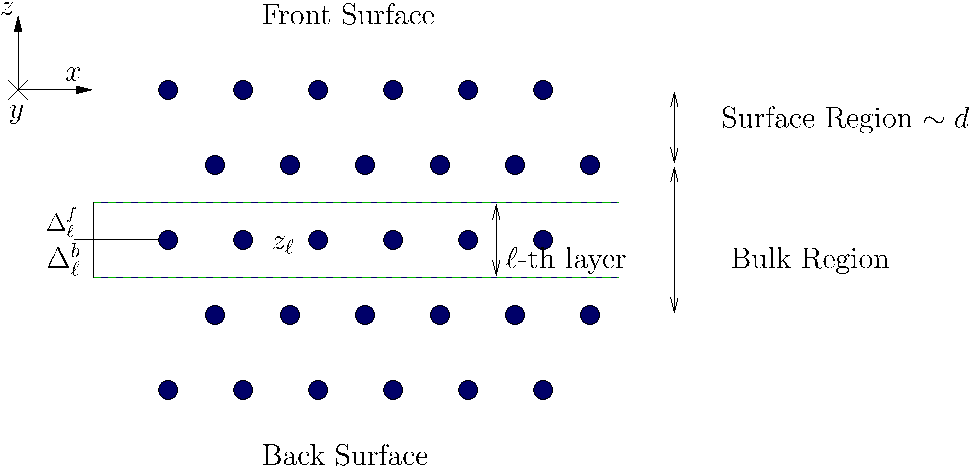
\includegraphics[height=5cm,width=7cm]{slab}
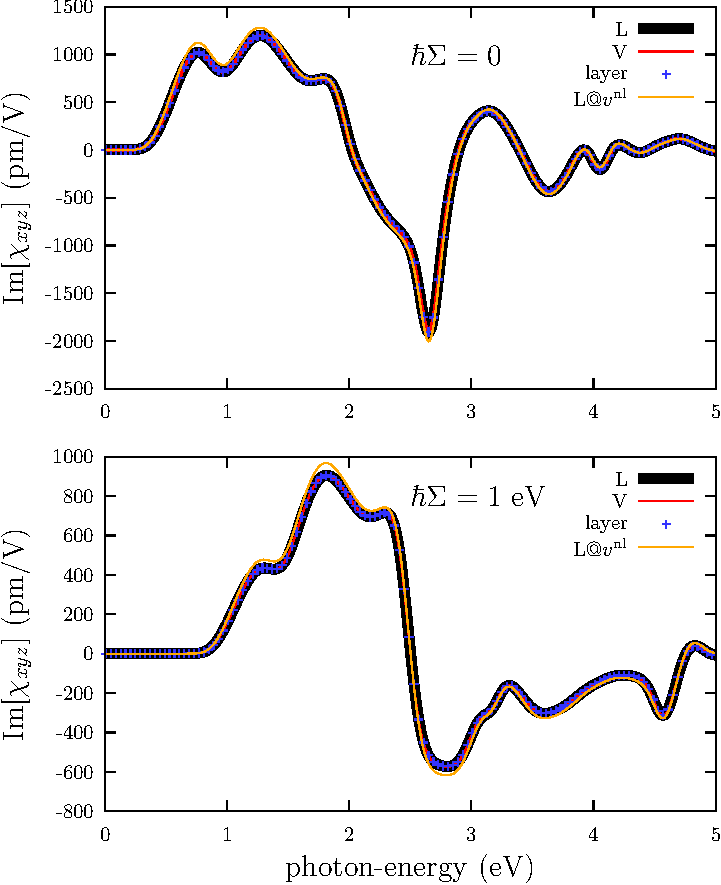
\includegraphics[scale=.7]{plots/shg-bulk}
\caption{Im[$\chi_{xyz}$] for GaAs, 10 Ha and 47 $\bfk$-points, using
  the layered formulation and mimicking a bulk. Also, the correction
  due to $\bfv^\nl$, which agree with the velocity and the layered
  approach (not shown).}
\label{gaas}
\end{figure}


\subsection{Consistency check-up 2}

To check that the coding of 
$\calc^\ell_{nm}(\bfk)$ 
is correct, we can calculate $\calv^{\rma,\ell}_{nm}(\bfk)$ using
Eq.~\eqref{vcali} as follows
\begin{align}\label{ccu.1}
\calv^{\rma,\ell}_{nm}(\bfk)
&=
\frac{1}{2m_e}
\Big(
\calc^\ell(z)p^\rma
+
p^\rma\calc^\ell(z)
\Big)_{nm}
\nonumber\\
&=
\frac{1}{2m_e}
\sum_q
\Big(
\calc^\ell_{nq}p^\rma_{qm}
+
p^\rma_{nq}\calc^\ell_{qm}
\Big)
,
\end{align}
which must give the same results as those computed through
Eq.~\eqref{eni.2}.
Indeed, we have checked that this is the case. The
\verb=$TINIBA/util/consistency-of-cfmn.sh=
is used to check this.

\subsection{Subroutines}

The following subroutines/shells are involved in the coding,
and are documented between\\
\verb=#BMSd=\\
$\vdots$\\
\verb=#BMSu=\\
marks.
\begin{enumerate}
\item \verb=$TINIBA/utils/all_responses.sh=
\item \verb=$TINIBA/latm/SRC_1setinput/inparams.f90=\\
\textcolor{red}{Warning:} compile both\\
\verb=$TINIBA/latm/SRC_1setinput/= \\
and\\
\verb=$TINIBA/latm/SRC_2latm/= 
\item \verb=$TINIBA/latm/SRC_1setinput/set_input_ascii.f90=\\
\end{enumerate}
